%Template v.1.0: Taylor Arnold and Simon Gabay, december 2025
% CECI EST UN FICHIER DE MODÈLE LATEX POUR LES ARTICLES INCLUS DANS
% *Anthology of Computers and the Humanities*. AJOUTEZ L'OPTION
% 'final' LORS DE LA CRÉATION DE LA VERSION FINALE DE L'ARTICLE. 
% NE PAS modifier la classe du document
\documentclass[final, fra]{anthology-ch}     % pour la version finale
%\documentclass[fra, custom]{anthology-ch}      % pour la soumission

% CHARGER LES PACKAGES LaTeX
\usepackage{booktabs}
\usepackage{graphicx}

% AJOUTEZ vos propres packages avec \usepackage{}
\usepackage{rotating}

% TITRE DE LA SOUMISSION
% Remplacez ceci par le titre de votre soumission
\title{Diagrammes de Sankey et réseaux pour comparer les éditions d'un recueil de textes}

% INFORMATIONS SUR LES AUTEURS ET LES AFFILIATIONS
% Pour chaque auteur, utilisez une nouvelle commande \author, avec
% les numéros entre crochets indiquant les affiliations correspondantes
% (section suivante) et l'ORCID-ID pour chaque auteur.  
\author[1]{Blanche d'Aubigny}[
  email=blanche.daubigny@gmail.com
]
\author[2]{Philippe Gambette}[
  orcid=0000-0001-7062-0262,
  email=philippe.gambette@univ-eiffel.fr
]


% Il doit y avoir un appel à \affiliation pour chaque affiliation des auteurs.
% Plusieurs affiliations peuvent être attribuées à un auteur
% et une affiliation peut être attribuée à plusieurs auteurs. 
\affiliation{1}{Sorbonne Université, CNRS, CELLF, Paris, France}
\affiliation{2}{Université Gustave Eiffel, CNRS, LIGM, Marne-la-Vallée, France}

% MOTS-CLÉS
% Fournissez un ou plusieurs mots-clés séparés par des virgules
% en utilisant les commandes suivantes
\keywords[fra]{génétique des recueils, réseaux de textes, diagrammes de Sankey, tau de Kendall}
\keywords[eng]{text collection genetics, text networks, Sankey diagrams, Kendall's tau}

% MÉTADONNÉES DE LA PUBLICATION
% Ces champs seront remplis lors de la publication ; 
% ils peuvent être laissés par défaut lors de la soumission
\pubyear{2026}
\pubvolume{4}
\pagestart{189}
\pageend{196}
\paperorder{23}
\conferencename{Actes de la Conférence Humanistica}
\conferenceeditors{Serena Crespi, Simon Gabay, Martin Grandjean, Ariane Pinche, Marie Puren et Léa Saint-Raymond}
\doi{10.63744/lyzeb0Ak2YKc}
\customhead{}

\addbibresource{bibliography.bib}

%%%%%%%%%%%%%%%%%%%%%%%%%%%%%%%%%%%%%%%%%%%%%%%%%%%%%%%%%%%%%%%%%%%%%%%%%%%
% DÉBUT DU TEXTE
\begin{document}

\maketitle

\begin{abstract}
%Nous nous intéressons, dans cet article, à la problématique d'interprétation des changements d'ordre entre éditions successives d'un recueil de textes : correspondent-ils à une réorganisation aléatoire ou montrent-ils certaines régularités, qui peuvent conduire à des hypothèses interprétatives ?
%Nous proposons une interface web permettant de visualiser ces changements d'ordre par des diagrammes de Sankey (réseaux dont les arêtes ont des épaisseurs distinctes) enrichis pour visualiser divers éléments de structure des éditions comparées. Ces visualisations peuvent être combinées pour analyser plus de deux éditions successives et enrichies par des fonctionnalités interactives en vue de fournir une comparaison multi-échelles, allant de l'ordre des textes dans les éditions du recueil aux différences de contenus entre les textes eux-mêmes. Quelques exemples tirés de l'{\oe}uvre poétique de Marceline Desbordes-Valmore  illustrent l'intérêt de ces outils d'exploration numérique pour la génétique des recueils.
In this article, we focus on the interpretation of order changes in successive editions of a collection of texts: do these changes reflect a random rearrangement or do they reveal certain patterns that might lead to interpretive hypotheses?
We provide a web interface that allows users to visualize these changes in order using Sankey diagrams (networks with edges of varying thickness), enhanced to display other structural characteristics of the compared editions. These visualizations can be combined to analyze more than two successive editions, and enhanced with interactive features to provide a multi-scale comparison, ranging from the order of texts within the collection, to differences in content between the texts themselves. A few examples drawn from the poetic works of Marceline Desbordes-Valmore illustrate the value of these digital exploration tools for text collection genetics.
\end{abstract}

\section{Introduction} 
Gérard Genette considère dans \emph{Seuils} que dans un recueil de poèmes brefs, {\guillemotleft} l’effet de séquence ou de progression est habituellement très faible, et l’ordre est le plus souvent arbitraire {\guillemotright}~\cite{Genette1987}. Dans le cas où des recueils de poèmes, ou de textes d'autres genres littéraires (nouvelles, maximes, contes, fables, etc.) présentent des ordres différents dans leurs éditions successives, s'agit-il de réorganisations arbitraires ou existe-t-il des critères, tenant par exemple à la progression globale du recueil, ou à des contraintes structurelles plus locales, pour expliquer les différences d'ordre ?

Dans cette contribution, nous montrons de quelle manière des outils de visualisation de réseaux peuvent aider à explorer ces questions. Nous proposons des interfaces web qui permettent à la fois une observation globale des changements d'ordre entre deux versions d'un recueil de textes, et des focus sur des phénomènes plus locaux liés par exemple à la structuration du recueil en parties. Ces interfaces peuvent facilement être générées à partir des tables des matières de deux éditions d'un recueil, organisées dans un document tableur.

\section{Visualisations de changements d'ordre}\label{sec:litterature}

Les outils de visualisation et d'analyse de données tels que les plateformes web RAWGraphs~\cite{Mauri2017} et NetSage~\cite{Schopf2022} proposent des visualisations en réseaux connues en anglais sous le nom de \emph{slope graphs} pour visualiser les différences d'ordre entre deux listes contenant les mêmes éléments, ou de \emph{bump charts} quand il s'agit de représenter l'évolution des différences d'ordre sur plus de deux listes d'éléments~\cite{Tufte2011}.

Dans le cas où l'on souhaite également représenter des évolutions de taille de ces éléments ordonnés, on peut avoir recours à des \emph{diagrammes alluviaux}~\cite{Mauri2017}, aussi appelés \emph{diagrammes de flux Sankey}~\cite{Schopf2022}. Ces derniers ont déjà été utilisés en humanités numériques pour représenter visuellement les différences entre deux éditions de \emph{Cloud Atlas} de David Mitchell mettant en relief des réorganisations de plusieurs segments du roman~\cite{Eve2016}. Nous proposons ici de faciliter leur construction pour des recueils de textes tout en tirant pleinement parti d'une visualisation interactive, et de la coloration, pour faciliter l'analyse des différences d'ordre et de contenu entre les recueils\footnote{Nous remercions Caroline Trotot et Christine Planté pour leurs retours sur des versions préliminaires de ces outils de visualisation interactive, qui ont permis de les améliorer.}.

\section{Corpus utilisés}\label{sec:corpus}

Nous nous intéressons à deux corpus de textes de Marceline Desbordes-Valmore. Le premier est constitué par les éditions de 1920 et de 1927 de l'anthologie de poèmes de Marceline Desbordes-Valmore (1786-1859) traduits en allemand, en annexe de la biographie de la poète par Stefan Zweig, intitulée~\emph{Marceline Desbordes-Valmore : das Lebensbild einer Dichterin}~\cite{Zweig1920App,Zweig1927App}.

Le second est constitué par les premiers recueils de poèmes de Marceline Desbordes-Valmore, publiés de 1819 à 1830~\cite{Desbordes1819,DesbordesValmore1820,DesbordesValmore1822,DesbordesValmore1825,DesbordesValmore1830}. 
Paru en 1819, le premier recueil au titre programmatique, \emph{Élégies, Marie et romances}, s’organise en trois sections, autour de la nouvelle « Marie ». Celle-ci comprend huit pièces versifiées, qui disparaissent définitivement dans l’édition suivante. Le recueil des \emph{Poésies} de 1820 conserve les élégies et les romances de 1819, à l'exception de «~Médor~», et leur adjoint vingt-quatre nouveaux poèmes. Les \emph{Poésies} de 1822 retranchent deux autres romances («~Le Réveil créole~» et «~Jone et Sophie~») et l’édition est augmentée de seize créations. En 1825, paraissent les \emph{Élégies et Poésies nouvelles}, où figurent cinquante-sept pièces absentes des recueils précédents : vingt élégies, quatre idylles, vingt-trois romances, six contes et trois «~poésies diverses~». Dans le recueil collectif des \emph{Poésies} de 1830, seuls onze poèmes des éditions de 1822 et 1825 ne sont pas repris et soixante-deux nouveaux apparaissent. Au cours des éditions successives, certaines « élégies » deviennent des «~idylles~», d’autres sont déplacées dans la catégorie «~mélanges~», qui est ensuite renommée «~poésies diverses~» et où l’on retrouve des poèmes auparavant classés parmi les «~contes~». 

L'ordre des poèmes dans ces recueils n'a pour le moment pas fait l'objet d'une étude approfondie, alors que, publié un an avant les \emph{Méditations poétiques} de Lamartine, %~\cite{Lamartine1820},
\emph{{\'E}légies, Marie et romances} occupe une place particulière dans le mouvement romantique français en poésie~\cite{Newkirk1954,Plante2011}. La correspondance de Marceline Desbordes-Valmore indique qu'après avoir confié à son éditeur François Louis la tâche d'ordonner les poèmes dans ce premier recueil, dans une lettre du 26 avril 1818, elle fixe, dans une autre lettre au même destinataire, le 3 octobre 1818, l'ordre des élégies~\cite{Cavallucci1936}.
Dans sa critique dans les \emph{Annales de la littérature et des arts}, en 1821, Jacques Ancelot déplore l'absence d'une progression dans la deuxième édition du recueil~\cite{Ancelot1821}, ce qui a pu pousser la poète à revoir de nouveau en profondeur l'ordre des poèmes dans l'édition suivante publiée l'année suivante.

Par ailleurs, dans son étude sur le cycle des poèmes à Délie dans ces recueils~\cite{DixonYoung2025}, Edie Dixon-Young accorde une attention particulière au déplacement en première position, à partir de 1822, du poème auparavant deuxième~\cite{DixonYoung2025}. Elle indique que pour privilégier l'un ou l'autre des deux ordres concurrents, les précédentes études de ces poèmes~\cite{Bertrand1973,Ambriere1987} s'étaient surtout fondées sur des considérations biographiques, comme cela est aussi fait dans un article évoquant l'ordre des poèmes d'\emph{{\'E}légies, Marie et romances}~\cite{Michel2010}. Elle-même se fonde sur des considérations esthétiques pour montrer les contrastes entre les deux premiers poèmes du cycle (quel que soit leur ordre) et le troisième.

\section{Méthodologie}\label{sec:methodologie}

\subsection{Un outil de comparaison de deux recueils de textes par un diagramme de Sankey}
Nous proposons d'une part une interface web, codée sous licence libre en HTML, CSS et Javascript~\footnote{\url{https://philippegambette.github.io/txtCompare/sankeyCompare}.}, pour représenter deux éditions d'un même recueil de textes par un diagramme de Sankey facilitant l'analyse des différences d'ordre des textes. Les données relatives au contenu des deux éditions sont structurées dans un document tableur : elles peuvent être établies directement à partir de la table des matières, en repérant ensuite manuellement, ou semi-automatiquement à partir des titres, à quel texte de la première édition correspond éventuellement chaque texte de la seconde.

Comme dans~\cite{Eve2016}, chaque recueil est alors représenté par un ensemble de rectangles verticaux, qui chacun représente un texte du recueil : la hauteur du rectangle dépend de la longueur du texte et les rectangles correspondant aux deux versions du texte dans les deux éditions du recueil sont reliées. Nous ajoutons la possibilité de répartir les textes en catégories, représentées par des couleurs dans la visualisation, qui peuvent correspondre à des parties du recueil ou à d'autres spécificités des textes.

Un formulaire permet de charger les URL de deux fichiers au format CSV, l'un pour indiquer les données relatives aux deux versions du recueil, l'autre pour les métadonnées relatives à ces deux versions. Un permalien intégrant les URL des deux fichiers CSV permet alors la diffusion des visualisations ainsi générées à partir des fichiers chargés.

\subsection{Une visualisation en réseau des premiers recueils de poèmes de Desbordes-Valmore}

Pour représenter les recueils de poèmes de Desbordes-Valmore publiés de 1819 à 1830, nous choisissons de généraliser le principe du diagramme de Sankey aux ensembles de recueils successifs. Mais nous le simplifions en uniformisant épaisseur des liens et taille des points représentant les textes\footnote{\url{https://philippegambette.github.io/txtCompare/recueilsMDV}.}, pour plus de lisibilité. Le recueil \emph{{\'E}légies, Marie et romances} (1819) apparait donc comme un ensemble horizontal de points qui représentent les poèmes qu'il contient. Les éditions suivantes de ce recueil, les \emph{Poésies} de 1820 et de 1822, 
adoptent la même forme, en dessous, tout comme les \emph{{\'E}légies et poésies nouvelles} de 1825,
qui ne contiennent que des poèmes inédits et les \emph{Poésies} de 1830 en deux tomes réunissant le tout, 
avec de nouveau des poèmes inédits réunis pour l'essentiel à la fin du deuxième tome, donc en bas à droite de la visualisation.

\begin{sidewaysfigure}[!htb]
  \centering
  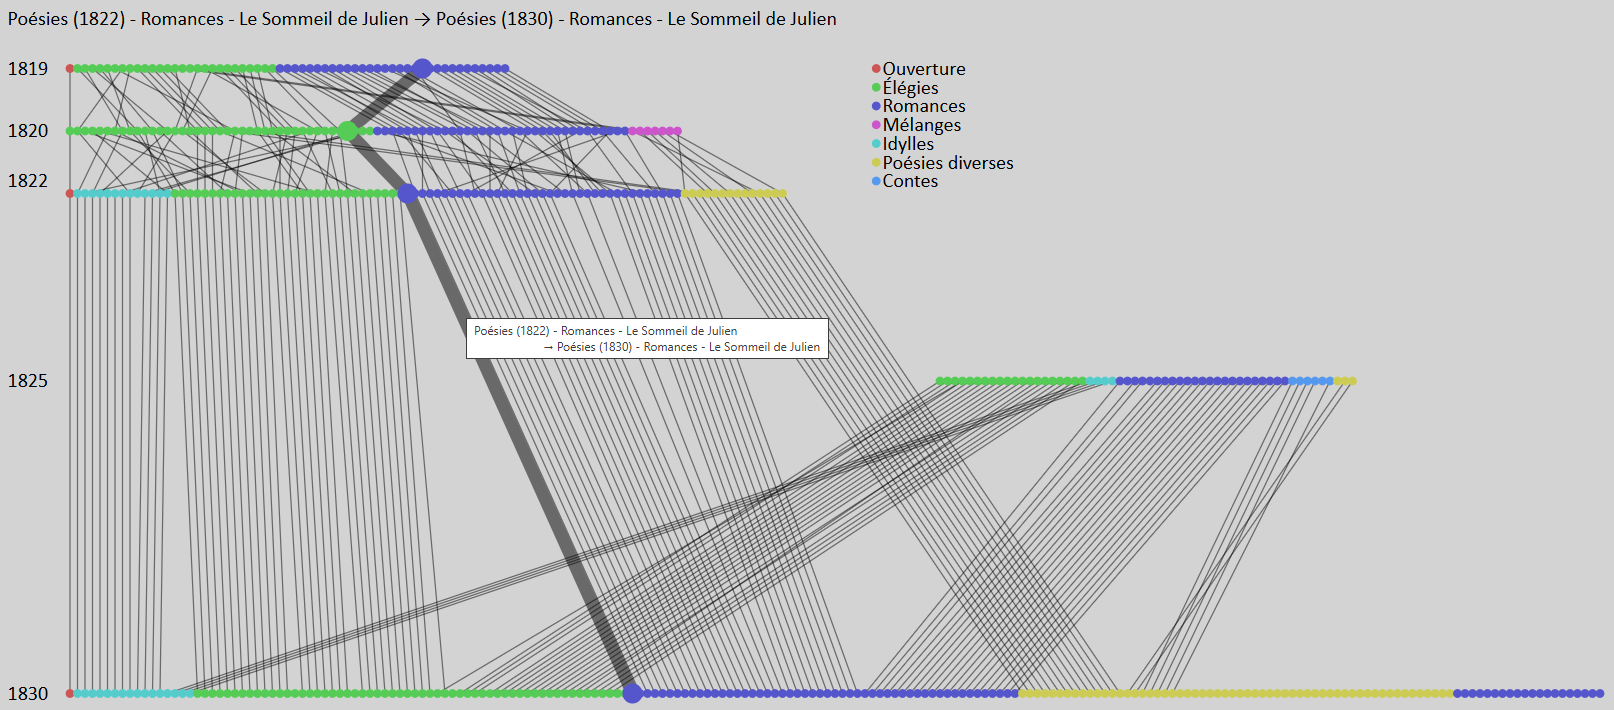
\includegraphics[width=\linewidth]{img/DesbordesValmore-Recueils.png}
  \caption{Visualisation des recueils de Marceline Desbordes-Valmore publiés entre 1819 et 1830. }
  \label{fig:recueils}
\end{sidewaysfigure}

Nous proposons une visualisation interactive, en permettant, par le survol avec la souris d'un lien reliant deux éditions successives d'un poème, de mettre en gras tous les liens situés entre éditions successives de ce poème. Les titres de ces deux versions liées par le lien survolé sont alors affichés en haut de la visualisation. Passer la souris sur un point coloré correspondant à un poème permet d'en lire le titre et d'épaissir les liens qui le relient à ses éditions dans les autres recueils. Cliquer sur ce point permet d'accéder à une version en ligne du texte du poème, et cliquer sur un lien ouvre une comparaison entre les deux versions du poème (utilisant parfois le texte obtenu par reconnaissance automatique de caractères, non relu), sous forme d'un alignement automatique construit avec le logiciel MEDITE~\cite{Sellami2015}, appelé de façon répétée grâce à un script Python~\footnote{\url{https://github.com/PhilippeGambette/txtCompare/tree/master/pairwiseMedite}.}.

\section{Résultats et discussion}\label{sec:resultats}

Dans la visualisation en diagramme de Sankey du premier corpus, montrée en figure~\ref{fig:zweig}\footnote{Version interactive sur \url{https://philippegambette.github.io/txtCompare/sankeyCompare/?id=4}.}, la couleur cyan indique les titres des poèmes de l'anthologie en annexe de la biographie de Marceline Desbordes-Valmore (1786-1859) publiée en 1921 par Stefan Zweig, qui ne sont pas repris dans la réédition de 1927. De même, sont colorées en bleu deux nouvelles traductions, dues à Friderike Zweig. La couleur des liens est automatiquement assombrie si le titre diffère, ce qui permet de détecter une seule variante de titre, l'ajout de la précision «~(vor seiner Reise in das Pensionat)~» au poème «~An meinen Sohn~». La visualisation montre un nombre conséquent de différences d'ordre, qui sont analysées par Ina Schabert comme une volonté de suivre davantage la thématique biographique du texte de Zweig, au détriment d'éléments plus variés de l'{\oe}uvre de Desbordes-Valmore qu'avait choisis la traductrice Etzel-Kühn, décédée peu après la publication de la première édition~\cite{Schabert2025}.

\begin{figure}[!htb]
  \centering
  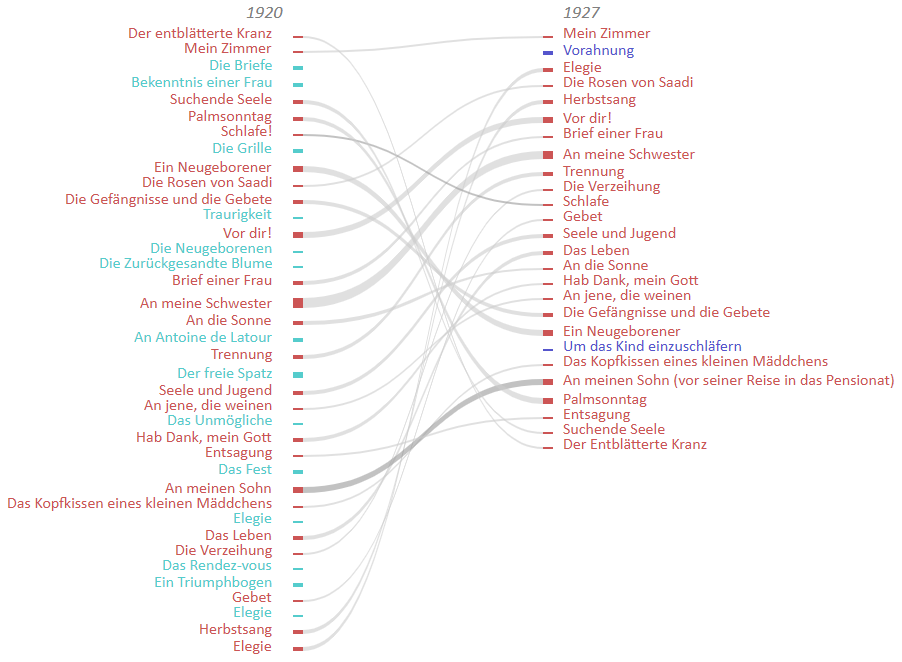
\includegraphics[width=\linewidth]{img/Zweig.png}
  \caption{Visualisation en diagramme de Sankey des éditions de 1920 et de 1927 de l'anthologie de poèmes en annexe de l'ouvrage de Stefan Zweig \emph{Marceline Desbordes-Valmore: das Lebensbild einer Dichterin}.}
  \label{fig:zweig}
\end{figure}

Nous avons choisi dans la capture d'écran de la figure~\ref{fig:recueils} de mettre en relief l'évolution de la place du poème «~Le Sommeil de Julien~» pour montrer qu'il est d'abord publié comme une romance située plutôt en fin de recueil, avant de devenir une des dernières élégies en 1820, puis de devenir la première romance des recueils à la fois de 1822 et de 1830. 
L'utilisation des couleurs pour indiquer les sections génériques de ces divers recueils (qui n'apparaitront plus dans les recueils suivants de la poète) permet donc de mettre en évidence la fluidité générique de certaines élégies de 1819 et 1820 qui deviennent idylles à partir de 1822.

De même, les cinq contes en vers repris du recueil de 1825 ne sont plus distingués des autres poésies diverses de 1830, même s'ils restent placés de façon contigüe, dans le même ordre. Cela peut conduire à lire comme des contes les poèmes placés juste avant, tirés des poésies diverses de l'édition de 1822, «~Conte imité de l’arabe~», «~La Mouche bleue~», «~L’Écolier~» et «~Conte d’enfant~», ou de l'édition de 1825, «~Le Billet d'une amie~» et «~L'Autruche et le Pélican~».

Parmi ces six poèmes, c'est peut-être pour «~Le Billet d'une amie~» que ce genre peut sembler le plus surprenant, en apportant justement une autre expérience de lecture. Les différences entre le texte des deux éditions du poème, visibles en cliquant sur le lien entre ces deux éditions, montrent un changement dans le dernier vers : «~Je le déteste{\ldots} eh quoi ! l’aimais-je encor ?~» devient «~Je hais l’amour{\ldots} Eh quoi ! l’aimais-je encor ?~». Alors que le pronom «~le~» de l'édition de 1825 pouvait être ambigu à la lecture des vers précédents (désigne-t-il l'amour, ou l'amant qui a trahi ?), la version de 1830 écarte la seconde hypothèse. Elle introduit en revanche une ambigüité sur le pronom «~l'~» final, autorisant une lecture plus générale du dernier vers («~aimais-je encore l'amour ?~») qui sonne alors comme une morale à ce conte.

\section{Conclusion et perspectives}

L'exemple complexe des premiers recueils de poèmes de Marceline Desbordes-Valmore montre comment les outils de visualisation présentés dans cette contribution combinent plusieurs possibilités de lecture, guidée par les couleurs ou par l'exploration à la souris des fonctionnalités d'interactivité et de retour au texte, pour des analyses approfondies des variations d'ordre. Il montre aussi de façon plus globale et percutante, par les segments parallèles, comment l'ordre des poèmes des éditions de 1822 et 1825 est stabilisé en 1830 : après les hésitations, parfois empreintes de modestie, sur l'ordre des premiers recueils de 1819 et 1820, Marceline Desbordes-Valmore n'est plus une actrice qui écrit des vers, mais une poète qui confirme ses choix de structuration en recueils.

Il pourrait être intéressant de déterminer à quel point les perturbations d'ordre que l'on peut constater sur les visualisations conservent l'ordre initial des textes du recueil, ou au contraire, tendent tout particulièrement à le renverser. Des fonctionnalités de calcul statistique pourraient alors être ajoutées dans l'interface, si l'on se limite à analyser les textes du premier recueil qui ont été repris, de façon unique, dans le second recueil : ceci permet de modéliser la différence entre les deux ordres par une permutation, dont il est alors possible de compter le nombre d'inversions, c'est-à-dire le nombre de paires de textes qui ont vu leur ordre s'inverser. Ce nombre pourra alors être comparé avec la distribution des nombres d'inversions de permutations aléatoires pour déterminer si l'ordre initial, ou l'ordre inverse, est plus conservé dans le second ordre des textes que ce qu'on pourrait attendre si le nouvel ordre avait été tiré au hasard. Le \emph{tau} de Kendall~\cite{Kendall1938}, qui fournit un score compris entre -1 et 1, proche de 1 en cas de respect de l'ordre original, et proche de -1 en cas de proximité avec l'inverse de l'ordre original, pourrait aussi, plus simplement, être calculé.

% Imprime la bibliographie à la fin. Gardez cette ligne après le texte
% principal de votre article et avant une annexe.
\printbibliography

% Vous pouvez inclure une annexe en utilisant la commande suivante
\appendix

\section{Annexes} \label{appdx:first}

\subsection{Extraits de la correspondance de Marceline Desbordes-Valmore et d'une critique à propos de l'ordre des poèmes dans ses premiers recueils}

Extrait d'une lettre du 26 avril 1818 de Marceline Desbordes-Valmore à son éditeur François Louis : «~Je m’en remets à vous seul du soin de classer par ordre chaque pièce de vers – elles sont copiées pêle-mêle – je n’ai pas eu la patience de choisir leur place. Donnez-leur le rang qu’il vous plaira, et le titre qui leur convient car l’auteur de tout cela est un peu comme Monsieur Jourdain qui fait de la prose sans le savoir.~»~\cite{Cavallucci1936}

Extrait d'une lettre du 3 octobre 1818 de Marceline Desbordes-Valmore à son éditeur François Louis : «~[...] j’ai cru qu’il fallait mettre les élégies dans l’ordre que je vous envoie par numéros ;~»~\cite{Cavallucci1936}

Extrait de la critique de Jacques Ancelot dans les \emph{Annales de la littérature et des arts}, en 1821 : «~Un recueil d'élégies est ordinairement un petit roman qui a son exposition, son action, son dénoûment : cette marche plaît au lecteur qui aime à rencontrer un fil qui le guide parmi ces morceaux détachés ; elle est surtout favorable à \emph{l'unité}, si précieuse à conserver en quelque chose qu'on écrive : M\textsuperscript{me} Desbordes n'a pas suivi cette méthode. Ses élégies, qui paraissent presque toutes avoir été inspirées par un même sentiment, n'ont cependant aucune suite entre elles ; un raccommodement précède une rupture, et à des plaintes sur l'inconstance d'Olivier, succède un éloge de sa fidélité. Dans une des élégies adressées à \emph{Délie}, M\textsuperscript{me} Desbordes lui adresse les plus vifs reproches ; dans la suivante, elle l'engage à venir pleurer au tombeau de son fils. Peut-être des motifs que nous ignorons ont pu engager l'auteur à mettre dans son ouvrage cette apparente confusion, mais elle peut être certaine que ce désordre ne paraît pas au lecteur \emph{un effet de l'art}.~»~\cite{Ancelot1821}
\end{document}